\section{Implementación de Pruebas}

Para garantizar el correcto funcionamiento de la aplicación, durante el desarrollo se ha realizado una fase de pruebas. Principalmente se han implementado pruebas unitarias, pero también algunas pruebas de integración para verificar el comportamiento de ciertos componentes y su interacción con los componentes vecinos.

\subsection{Framework y Librerías}

Para la ejecución de los tests se ha utilizado \textbf{Jest} como framework principal, junto con \textbf{React Testing Library} para la prueba de componentes de \textit{React}. Jest permite ejecutar tests de forma rápida y aislar cada prueba en un entorno controlado, mientras que \textit{React Testing Library} facilita la interacción y consulta de elementos en el DOM, asegurando que los tests reflejen mejor el comportamiento real de los usuarios.

En el caso de los endpoints del backend, \textit{Next.js} no proporciona un mecanismo directo para testear las API definidas con \textit{Route Handlers}, por lo que ha sido necesario el uso de la librería \textbf{\texttt{next-test-api-route-handler}}. Esta herramienta permite simular peticiones HTTP a los endpoints del backend y verificar las respuestas esperadas, facilitando la validación del comportamiento de la lógica del servidor.

\subsection{Consideraciones a Tener en Cuenta}

A la hora de escribir los tests, se han tenido en cuenta diferentes aspectos para asegurar su correcta ejecución:

\begin{itemize}
    \item \textbf{Entorno de ejecución}: Jest permite definir diferentes entornos de ejecución, siendo los más relevantes \textit{jsdom}, que simula un entorno de navegador, y \textit{node}, que representa el entorno de servidor. En este proyecto, \textbf{se han utilizado ambos entornos} según corresponda, ya que existen tanto componentes de cliente como de servidor. Es importante indicar explícitamente el entorno en la configuración de Jest para evitar errores en la ejecución de los tests.

    \item \textbf{Configuración de variables de entorno}: Algunas pruebas requieren acceso a variables. Para ello, se ha utilizado el archivo \textbf{\texttt{.env.test}}, donde se definen las variables necesarias en el contexto de pruebas.

    \item \textbf{Cobertura del código}: Se ha utilizado la funcionalidad de cobertura de Jest para analizar qué partes del código están siendo verificadas por las pruebas y detectar posibles áreas sin testear.
\end{itemize}

Además de la ejecución local de las pruebas, se ha configurado un flujo de integración continua (CI) para ejecutar los tests automáticamente en cada nueva actualización del código. Esto se ha realizado mediante \textbf{GitHub Actions}, asegurando que cualquier cambio en el proyecto sea validado antes de desplegarse. Se explican más detalles sobre esta integración en el capítulo de Despliegue, en la sección \nameref{sec:test_automaticos}.

\subsection{Lista de Pruebas}

En esta sección se presenta un resumen de las pruebas realizadas para los componentes, utilidades y endpoints del backend de la aplicación. A continuación, se muestran los elementos evaluados junto con la cantidad de tests ejecutados sobre cada uno. Para una descripción detallada de cada prueba, se remitir al \hyperref[ch:anexoE]{Anexo E}, donde se incluye la lista completa con los tests específicos realizados para cada caso.

\begin{table}[H]
    \centering
    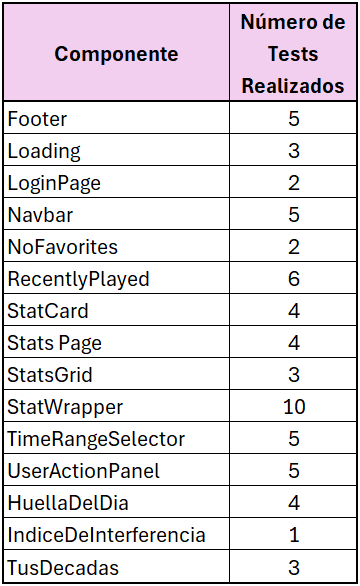
\includegraphics[width=0.4\textwidth]{figures/pruebas/numero_test_componentes.png}
    \captionsetup{skip=7pt}
    \caption{Número de pruebas ejecutadas por cada componente.}
    \label{tab:numero_test_componentes}
\end{table}

\begin{table}[H]
    \centering
    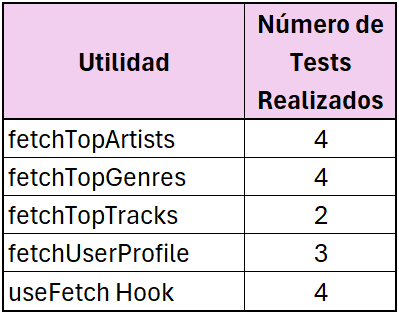
\includegraphics[width=0.4\textwidth]{figures/pruebas/numero_test_utilidad.png}
    \captionsetup{skip=7pt}
    \caption{Número de pruebas ejecutadas por cada utilidad.}
    \label{tab:numero_test_utilidad}
\end{table}

\vspace{-0.5cm}

\begin{table}[H]
    \centering
    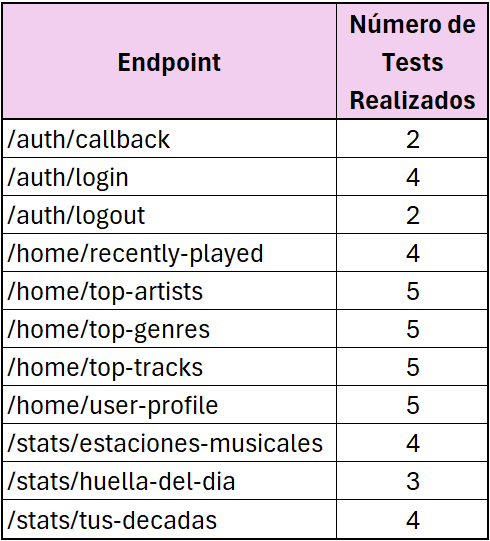
\includegraphics[width=0.45\textwidth]{figures/pruebas/numero_test_endpoints.png}
    \captionsetup{skip=7pt}
    \caption{Número de pruebas ejecutadas por cada endpoint de la API del backend.}
    \label{tab:numero_test_endpoints}
\end{table}

Se puede destacar que el componente (y elemento) con más tests realizados ha sido \textbf{StatWrapper}. Esto se debe a que es el componente encargado de renderizar en su interior todas las estadísticas avanzadas, por lo que es una pieza importante de la página web. Tiene muchas interacciones posibles, como formas de cerrar la ventana modal, y se realizan una variedad de pruebas para asegurarse de que el componente se muestra y se oculta de manera correcta, cuando esto deba ocurrir.

\newpage

\section{Resultados de Pruebas}

Tras la ejecución de las pruebas, se han obtenido los siguientes resultados globales:

\begin{table}[H]
    \centering
    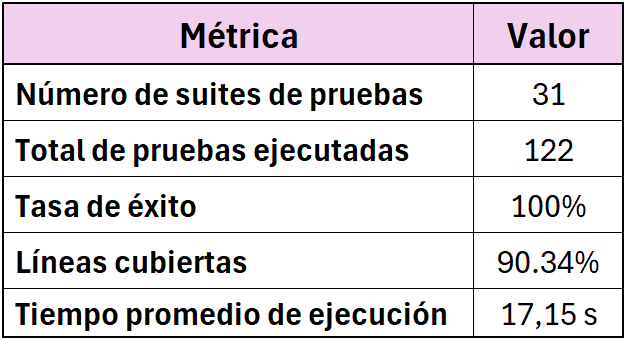
\includegraphics[width=0.5\textwidth]{figures/resultado_tests.png}
    \captionsetup{skip=7pt}
    \caption{Resultados globales de la ejecución de las pruebas.}
    \label{tab:resultado_tests}
\end{table}

\subsection{Interpretación de los Resultados}

La tasa de éxito del 100\% en las pruebas refleja que todas las verificaciones han pasado correctamente en cada ejecución. Sin embargo, \textbf{esto no significa que no se hayan encontrado problemas durante el desarrollo}. En varias ocasiones, los errores en los tests no estaban relacionados con fallos en la implementación de la aplicación, sino con limitaciones técnicas de Jest o con dependencias externas que dificultaban su correcta ejecución.

Uno de los principales obstáculos ha sido la incompatibilidad de ciertas librerías con Jest. Por ejemplo, los módulos basados en \textit{CommonJS}, como \texttt{D3.js}, han presentado dificultades en su integración con el entorno de pruebas. Además, los componentes que dependen de \texttt{canvas} no cuentan con soporte nativo en Jest, lo que impidió la ejecución de tests sobre algunos gráficos. Se intentó mitigar estos problemas mediante \textit{mocking} de dependencias, pero sin obtener resultados satisfactorios para todos los casos.

Aun así, la principal razón por la que se ha decidido suprimir los tests problemáticos ha sido por el flujo CI: Dado que está configurado en \textit{GitHub Actions} para ejecutar la suite de pruebas antes de cada despliegue en \textit{Vercel}, cualquier fallo en los tests bloquearía la actualización del código en producción. Para evitar interrupciones innecesarias en el despliegue debido a errores ajenos a la aplicación, se optó por retirar aquellas pruebas que no podían ofrecer resultados fiables sin comprometer la estabilidad del CI. A pesar de esta decisión, se ha garantizado que los tests implementados cubren los aspectos esenciales del sistema. Se han validado correctamente los endpoints del backend, la lógica de negocio y los principales componentes del frontend, asegurando que las funcionalidades críticas de la aplicación están correctamente verificadas. Para aquellos aspectos que no podían ser testeados automáticamente con Jest, como ciertos elementos gráficos o validaciones de autenticación, se han realizado pruebas manuales.

Finalmente, se ha trabajado en el tiempo de ejecución de las pruebas, logrando que la batería completa de 122 tests se ejecute en un promedio de 17.15 segundos. Este tiempo es aceptable, donde cada ejecución acumula tiempos entre la creación y configuración del entorno y la ejecución de los tests. Mantener este tiempo bajo control es un aspecto importarte en un flujo CI/CD.

\subsection{Cobertura del Código}

Por otro lado, también se ha utilizado la funcionalidad de cobertura de código de Jest para evaluar qué porcentaje del código está siendo verificado por los tests. La cobertura se mide en cuatro dimensiones:

\begin{itemize}
    \item \textbf{Statements}: Sentencias ejecutadas. \vspace{-5pt}
    \item \textbf{Branches}: Ramas de ejecución en estructuras de control (\textit{if/else}). \vspace{-5pt}
    \item \textbf{Functions}: Funciones llamadas. \vspace{-5pt}
    \item \textbf{Lines}: Líneas de código ejecutadas.
\end{itemize}

Los resultados en la tabla \ref{tab:coverage_tests} muestran que la mayoría de los archivos tienen una \textbf{cobertura superior al 90\%}, lo que indica que la mayor parte del código ha sido testeado de manera efectiva. No obstante, algunos archivos presentan una cobertura significativamente más baja:

\begin{itemize}
    \item \textbf{\texttt{app/api/auth/callback.ts}}: El archivo tiene una cobertura del 35.06\%. Esto se debe por el valor \texttt{state} que se utiliza para la protección ante ataques CSRF (\textit{Cross-Site Request Forgery}). Como no es el flujo de autenticación estándar, se genera un error \texttt{state\_mismatch} en todos los casos.
    \item \textbf{\texttt{components/stats/IndiceDeInterferencia.tsx}}:  Tiene una cobertura del 44.27\%, lo que indica que ciertas partes de la lógica de este componente aún no han sido probadas. En esta estadística es donde se hace uso de la librería D3.js, que genera problemas al no manejar módulos ESModules.
\end{itemize}

A pesar de estas limitaciones, la cobertura global es elevada y ha permitido validar el correcto funcionamiento de los principales módulos de la aplicación.

\begin{table}[htbp]
    \centering
    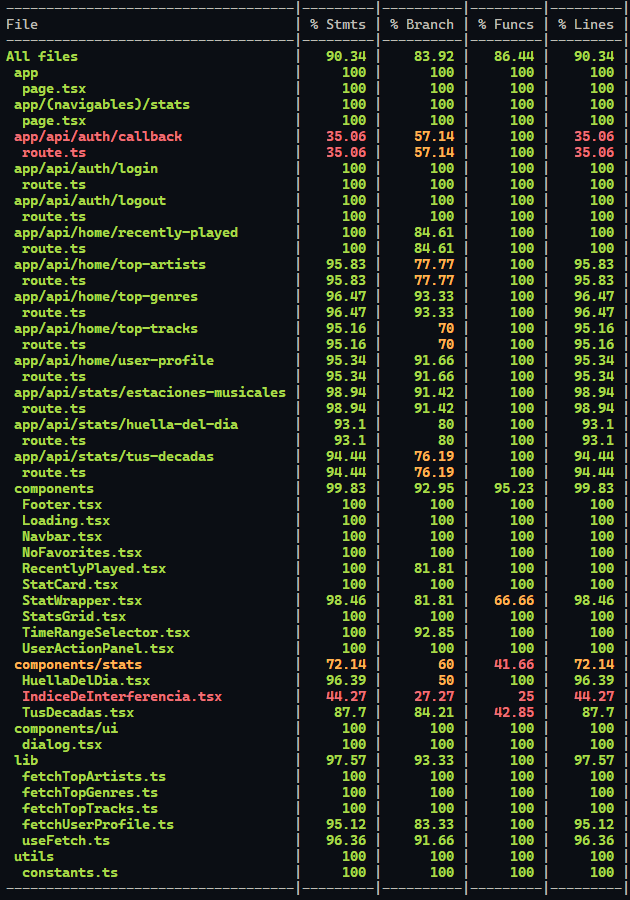
\includegraphics[width=0.65\textwidth]{figures/coverage_tests.png}
    \captionsetup{skip=7pt}
    \caption{Desglose generado por Jest de la cobertura del código del proyecto.}
    \label{tab:coverage_tests}
\end{table}


